%%%%%%%%%%%%%%%%%%%%%%%%%%%%%%%%%%%%%%%%%%%%%%%%%%%%%%%%%%%%%%%%%%%%%%%%
%
% Template latex file for a common article class for class notes
% and write ups. Additional Configuration and styling options are 
% commented out. ex. Table of Contents and Title page
% 
% Author: Amy Bui
%
%%%%%%%%%%%%%%%%%%%%%%%%%%%%%%%%%%%%%%%%%%%%%%%%%%%%%%%%%%%%%%%%%%%%%%%%

\documentclass[12pt]{article}
\usepackage[utf8]{inputenc}
\usepackage{parskip}
\usepackage{tabularx}
\usepackage{caption}
\usepackage{subcaption}
\usepackage[color, leftbars]{changebar}

% Important Configurations

%%%%%%%%%%%%%%%%%%%%%%%%%%%%%%%%%%%%%%%%%%%%%%%%%%%%%%%%%%%%%%%%%%%%%%%%
% Reduce margin
%
% \addtolength{\oddsidemargin}{-.85in}
% \addtolength{\evensidemargin}{-.85in}
% \addtolength{\textwidth}{1in}

% \addtolength{\topmargin}{-.85in}
% \addtolength{\textheight}{1in}

% Page format commands:
% Override normal article margins,
% making the margins smaller
\setlength{\textwidth}{6.5in}
\setlength{\textheight}{9in}
\setlength{\oddsidemargin}{0in}
\setlength{\evensidemargin}{0in}
\setlength{\topmargin}{-0.5in}

\setlength{\parindent}{0pt}
%%%%%%%%%%%%%%%%%%%%%%%%%%%%%%%%%%%%%%%%%%%%%%%%%%%%%%%%%%%%%%%%%%%%%%%%


%%%%%%%%%%%%%%%%%%%%%%%%%%%%%%%%%%%%%%%%%%%%%%%%%%%%%%%%%%%%%%%%%%%%%%%%
% Math Symbols
\usepackage{mathtools}
\usepackage{amssymb}
% \usepackage{epsfig}
\usepackage{amsmath,amsthm}
\usepackage{amscd,amsxtra,latexsym}


% add floor and ceiling symbol. Usage: \ceil*{}, \floor*{}
\DeclarePairedDelimiter\ceil{\lceil}{\rceil}
\DeclarePairedDelimiter\floor{\lfloor}{\rfloor}

% multiset \langle ... \rangle
\def\multiset#1#2{\ensuremath{\left(\kern-.3em\left(\genfrac{}{}{0pt}{}{#1}{#2}\right)\kern-.3em\right)}}



%%%%%%%%%%%%%%%%%%%%%%%%%%%%%%%%%%%%%%%%%%%%%%%%%%%%%%%%%%%%%%%%%%%%%%%%

%%%%%%%%%%%%%%%%%%%%%%%%%%%%%%%%%%%%%%%%%%%%%%%%%%%%%%%%%%%%%%%%%%%%%%%%
% Code Sample Styling

% use \lstinline! xxx ! or \begin{lstlisting} ... \end{lstlisting}
\usepackage{listings}

\usepackage{color}
\definecolor{light-gray}{gray}{0.97} % shade of grey
\definecolor{dkgreen}{rgb}{0,0.6,0}
\definecolor{gray}{rgb}{0.5,0.5,0.5}
\definecolor{mauve}{rgb}{0.58,0,0.82}

% \begin{lstlisting}[...] ... \end{lstlisting}
\lstset{frame=none,
    language=C++,
    aboveskip=3mm,
    belowskip=3mm,
    stepnumber=1, % set to 0 if you don't like line nums
    showstringspaces=false,
    columns=flexible,
    basicstyle={\small\ttfamily},
    numbers=left,
    numberstyle=\color{black},
    keywordstyle=\color{blue},
    commentstyle=\color{dkgreen},
    stringstyle=\color{mauve},
    backgroundcolor=\color{light-gray},
    breaklines=true,
    breakatwhitespace=false,
    tabsize=2
}



%%%%%%%%%%%%%%%%%%%%%%%%%%%%%%%%%%%%%%%%%%%%%%%%%%%%%%%%%%%%%%%%%%%%%%%%

%%%%%%%%%%%%%%%%%%%%%%%%%%%%%%%%%%%%%%%%%%%%%%%%%%%%%%%%%%%%%%%%%%%%%%%%
\usepackage{xcolor}
%% https://tex.stackexchange.com/questions/401750/quick-and-short-command-for-coloring-one-word
\newcommand\shorthandon{\catcode`@=\active \catcode`^=\active \catcode`*=\active }
\newcommand\shorthandoff{\catcode`@=12 \catcode`^=7 \catcode`*=12 }
\shorthandon
\def@#1@{\textcolor{red}{#1}}%
\def^#1^{\textcolor{blue}{#1}}%
\def*#1{\string#1}
\shorthandoff
%% useage: \textcolor{red}{text here}
% \shorthandon
% This is a @test@ of the ^emergency^ bro*@dcast system.
% \shorthandoff
%%%%%%%%%%%%%%%%%%%%%%%%%%%%%%%%%%%%%%%%%%%%%%%%%%%%%%%%%%%%%%%%%%%%%%%%


%%%%%%%%%%%%%%%%%%%%%%%%%%%%%%%%%%%%%%%%%%%%%%%%%%%%%%%%%%%%%%%%%%%%%%%%

%Commands below change page margins (this much space at the titlepage, etc)
\newlength{\toppush}
\setlength{\toppush}{2\headheight}
\addtolength{\toppush}{\headsep}

% Section header Styling
% The commands below change the bold text where it says "Section" into "Question"
% \usepackage{titlesec}
% \titleformat{\section}
% {\normalfont\Large\bfseries}{Question~\thesection:}{1em}{}

% I added this command below to chance "subsections numbers" to be "Question [subsection number]" -AB 1/31/2021
% \titleformat{\subsection}
% {\normalfont\bfseries}{\thesubsection:}{1em}{}

% Page head Styling
% Name and subject of the class
\def\subjnum{Comp 163}          % Class Number
\def\subjname{CompGeo}       % Class Name

% Name of the student, university name and which semester
\def\doheading#1#2#3{\vfill\eject\vspace*{-\toppush}%
  \vbox{\hbox to\textwidth{{\bf} \subjnum: \subjname \hfil Amy Bui}%
    \hbox to\textwidth{{\bf} Tufts University, Fall 2022 \hfil#3\strut}%
    \hrule}}

%Command for the title of the document (Homework 0)
\newcommand{\htitle}[1]{\vspace*{1.25ex plus 1ex minus 0ex}%
\begin{center}
    {\large\bf #1}
\end{center}} 
%%%%%%%%%%%%%%%%%%%%%%%%%%%%%%%%%%%%%%%%%%%%%%%%%%%%%%%%%%%%%%%%%%%%%%%%



%%%%%%%%%%%%%%%%%%%%%%%%%%%%%%%%%%%%%%%%%%%%%%%%%%%%%%%%%%%%%%%%%%%%%%%%
% Misc
\usepackage{graphicx} % graphics
\usepackage{enumitem} % listing style (bullet lists)

% below helps with trying to get figures in a row
% \usepackage{caption}
% \usepackage{subcaption}

% hyperlink styling
% use \href{} and \url{}, and colors table of contents links
% use \href{} and \url{}
% \label{sec:name}
% \hyperref[label]{text}
\usepackage{hyperref}
\hypersetup{
    colorlinks=true,
    linkcolor=blue, % was previously black
    filecolor=magenta,
    urlcolor=blue,
    pdftitle={Template}
}
\urlstyle{same}

% A command for primes (')
\newcommand{\p}%
    {\ensuremath{^{\prime}}}

% a command for double primes ('')
\newcommand{\pp}%
    {\ensuremath{^{\prime \prime}}}

% A command for the Kleene star
\newcommand{\str}%
    {\ensuremath{^{\star}}}

% a command for the double star
\newcommand{\sstr}%
    {\ensuremath{^{\star\star}}}
%%%%%%%%%%%%%%%%%%%%%%%%%%%%%%%%%%%%%%%%%%%%%%%%%%%%%%%%%%%%%%%%%%%%%%%%

% Options for title page, use \maketitle in document
% \author{Amy Bui}
% \title{COMP160 - Algorithms: Class Notes and Practice}

\begin{document}
%% create title page
% \title{(g)ROOT \\ Language Reference Manual}
% \author{Samuel Russo \quad Amy Bui \quad Eliza Encherman \\ Zachary Goldstein \quad Nickolas Gravel}
% \date{\today}
% \maketitle

\doheading{2}{title}{Notes}

    %%%%%%%%%%%%%%%%%%%%%%%%%%%%%%%%%%%%%%%%%%%%%%%%%%%%%%%%%%%%%%%%%%%%%%%%
    % Table of Contents
    \setcounter{tocdepth}{2}
    \tableofcontents
    \pagebreak
    %%%%%%%%%%%%%%%%%%%%%%%%%%%%%%%%%%%%%%%%%%%%%%%%%%%%%%%%%%%%%%%%%%%%%%%%

    %%%%%%%%%%%%%%%%%%%%%%%%%%%%%%%%%%%%%%%%%%%%%%%%%%%%%%%%%%%%%%%%%%%%%%%%
    \section{Algorithms: Overview}
    \label{sec:allalgo}

        \begin{center}
            \begin{tabular}{|p{3cm}|p{3.5cm}|p{2cm}|p{2cm}|p{2cm}|p{2.25cm}|}
                \hline
                \hline
                \textbf{TOPIC/type} & \textbf{Name} & \textbf{Best} & \textbf{Average} & \textbf{Worst} & \textbf{Space} \\ 
                \hline
                \hline
                \hyperref[sec:convexhull]{\textbf{Convex Hull}} & & $\Omega(n)$ & & $O(n^4)$ &  \\
                \hline
                incremental & \hyperref[subsec:chn4]{Naive Approach (Triples)} & $\Omega(n^4)$ & $\Theta(n^4)$ & $O(n^4)$ & \\
                \hline
                incremental & \hyperref[subsec:slowhull]{Slow $\mathcal{CH}$ (Pairs)} & $\Omega(n^3)$ & $\Theta(n^3)$ & $O(n^3)$ & \\
                \hline
                incremental & \hyperref[subsec:giftwrapping]{Jarvis March(Gift Wrapping)} & $\Omega(n h)$ & $\Theta(n \log n)$ & $O(n^2)$ & \\
                \hline
                incremental & \hyperref[subsec:gscan]{Graham Scan} & $\Omega(n \log n)$ & $\Theta(n \log n)$ & $O(n \log n)$ & \\
                \hline
                D\&C& \hyperref[subsec:quickhull]{Quick Hull} & $\Omega(n\log n)$ & $\Theta(n \log n)$ & $O(n^2)$ & \\
                \hline
                prune\&search& \hyperref[subsec:ultimatehull]{Marriage before Conquest (Ultimate)} & $\Omega(n \log h)$ & $\Theta(n \log h)$ & $O(n \log h)$ & \\
                \hline
                order decomp & \hyperref[subsec:dynamichull]{Dynamic Convex Hull} & $\Omega(\log^2 n)$ & $\Theta(\log^2 n)$ & $O(\log^2 n)$ & \\
                \hline
                \hyperref[]{\textbf{Intersecting Points}} & & $\Omega(?)$ & & $O(n^2)$ &  \\
                \hline
                & Naive (test every segment for intersections with each other) & $\Omega(n^2)$ & $\Theta(n^2)$ & $O(n^2)$ & \\
                \hline
                & Plane Sweep (sweep line) & $\Omega(?)$ & $\Theta(?)$ & $O(?)$ & \\
                \hline
                \hline
                & Name & $\Omega(n \log n)$ & $\Theta(n \log n)$ & $O(n \log n)$ & \\
                \hline
                & Kirkpatrick's Hierarchical Search && $\Theta(n \log n)$ &  & $O(n)$\\
                & & & & & \\
                \hline
                & Name & $\Omega(n \log n)$ & $\Theta(n \log n)$ & $O(n \log n)$ & \\
                \hline
                \hline
            \end{tabular}
        \end{center}

        \emph{h is the number of points on $\mathcal{CH}$.}

    \pagebreak
    %%%%%%%%%%%%%%%%%%%%%%%%%%%%%%%%%%%%%%%%%%%%%%%%%%%%%%%%%%%%%%%%%%%%%%%%

    %%%%%%%%%%%%%%%%%%%%%%%%%%%%%%%%%%%%%%%%%%%%%%%%%%%%%%%%%%%%%%%%%%%%%%%%
    \section{Intro: Computational Geometry - A User's Guide (Notes)}
    \label{sec:compgeointro}
    Introduction to algorithims for computations that are geometric in nature. Souvaine \& Dobkin describe some methods with geometric applications.

    Three families of Geometric Algorithms:
    \begin{itemize}
        \item Decomposition of problem into subproblems -- \hyperref[subsec:hsm]{Hierarchical Searching Method} 
        \item Decomposition of problem into subproblems -- \hyperref[subsec:dcm]{Divide and Conquer Method}
        \item Transform a problem into a new (maybe more tractable) format -- \hyperref[subsec:dualitym]{Duality Method}
    \end{itemize}

    Geometric Principles
    \begin{itemize}
        \item Planar Point Location
        \item Convex Hull Construction and Updating
        \item Computation of Polygon
        \item Computation of Disk
        \item Computation of Half-Space Intersections
    \end{itemize}

        %%%
        \subsection{Hierarchical Searching Method}
        \label{subsec:hsm}
            \begin{itemize}
                \item Geometric problem is preprocessed to a coarse representation, such that it can be broken down, and search queries can be called on localized region where the problem is solved. 
                \item Algorithmic efficiency is then balanced against preprocessing time and storage space requirements. 
                \item Binary Search of Sorted Array 
            \end{itemize}

            \subsubsection{\href{https://www.geeksforgeeks.org/binary-search/}{Binary Search} on Geometric Problems}
                \begin{description}
                    \item[Input:] A collection of $N$ disjointed polygons in the plane.
                    \item[Output:] For a given point $P$, find all polygons to which it belongs
                    \item[Naive Solution:] check for $P$ in each points of the polygons. 
                    \item[Rectangle Search I \& II \& III] 
                    \item[General \& Dynamic Polygon Search] 
                \end{description}

        %%%
        \subsection{Divide and Conquer Method}
        \label{subsec:dcm}
        \begin{itemize}
            \item Problem broken into smaller subproblems, and solved recursively. A method is defined for combining solutions to subproblems to come up with solution for entire problem.
            \item Sort-merge
            \item Can work with heierarchical search methods, e.g. divide-and-conquer to sort a set, and then use binary search to find target.
        \end{itemize}

        %%%
        \subsection{Duality Method}
        \label{subsec:dualitym}
            \begin{itemize}
                \item Duality is used as a transformation. Given two sets A and B and a problem about their interrelationship, apply transform T and solve the (ideally simpler) problem about T(A) and T(B).
            \end{itemize}
    \pagebreak
    % END %%%%%%%%%%%%%%%%%%%%%%%%%%%%%%%%%%%%%%%%%%%%%%%%%%%%%%%%%%%%%%%%%%%%

    %%%%%%%%%%%%%%%%%%%%%%%%%%%%%%%%%%%%%%%%%%%%%%%%%%%%%%%%%%%%%%%%%%%%%%%%
    \section{Convex Hull}
    \label{sec:convexhull}
    Covered in \cite{berg08} CH. 1.1

    HW 1
    
    %%%
    \subsection{Geometry of Convex Hull}
    \begin{figure}[h]
        \centering
        \begin{tabular}{cc}
            \begin{subfigure}{.5\textwidth}
                \centering
                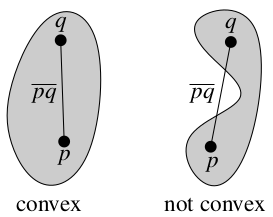
\includegraphics[width=0.5\linewidth]{images/convexhull1.png}
                \caption{}
                \label{fig:convexhull1}
            \end{subfigure} &
            \begin{subfigure}{.5\textwidth}
                \centering
                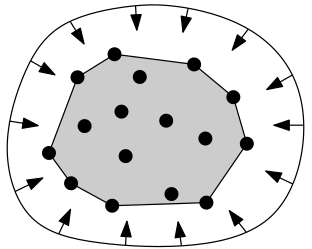
\includegraphics[width=0.5\linewidth]{images/convexhull2.png}
                \caption{}
                \label{fig:convexhull2}
            \end{subfigure}
        \end{tabular}
        \caption{Example of Convexity}
    \end{figure}

    \begin{itemize}
        \item The computation of \textbf{planar convex hull} was one of the first computational geomtry problems. 
        \item \emph{Convexity 1}: A subset $S$ of the plane is \textbf{convex} if and only if for any pair of points $p, q \in S$, the line segment $\overline{pq}$ is completely contained in $S$. See Fig. \ref{fig:convexhull1}. The \emph{convex hull}, $\mathcal{CH}(S)$, of a set $S$ is the smallest convex set that contains $S$; it is the intersection of all convex sets that contain $S$. 
        \item \emph{Convexity 2}: How to compute the convex hull of a finite set $P$ of $n$ points in the plane? The area enclosed in the shaded region is the convex hull of $P$. See Fig. \ref{fig:convexhull2}. It is the unique convex polygon whose vertices are points from $P$.
    \end{itemize}


    \begin{figure}[h]
        \centering
        \begin{tabular}{cc}
            \begin{subfigure}{.5\textwidth}
                \centering
                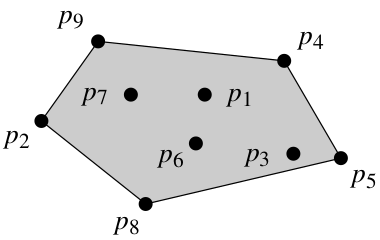
\includegraphics[width=0.5\linewidth]{images/convexhull3.png}
                \caption{}
                \label{fig:convexhull3}
            \end{subfigure} &
            \begin{subfigure}{.5\textwidth}
                \centering
                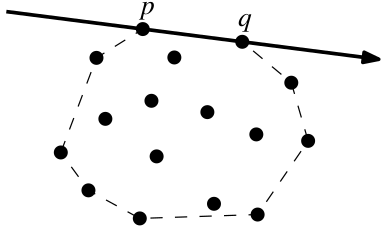
\includegraphics[width=0.5\linewidth]{images/convexhull4.png}
                \caption{}
                \label{fig:convexhull4}
            \end{subfigure}
        \end{tabular}
        \caption{computing convex hull}
    \end{figure}


    \begin{itemize}
        \item Fig. \ref{fig:convexhull3}: To compute a convex hull of a set of points, $P = \{p_1, p_2, ... p_9\}$, we compute a list of those vertices from $P$ that are the vertices of $\mathcal{CH}(P)$, i.e. $\{p_4, p_5, p_8, p_2, p_9\}$, and list them in clockwise order. Defining $\mathcal{CH}(P)$ as a convex polygon is more useful than discussing the intersection of all convex sets. 
        \item Fig. \ref{fig:convexhull4}: For points $p$ and $q$ that are endpoints of an edge and that are in $P$, we direct a line through $p$ and $q$, and if $\mathcal{CH}(P)$ lies to one side, then all points in $P$ must lie to that side of the $\overline{pq}$ line. And if all points of $P \setminus \{p, q\}$ lie to one side of $\overline{pq}$, then $\overline{pq}$ is an edge of the $\mathcal{CH}(P)$.
    \end{itemize}

    From Class, Algorithmic \textbf{Paradigms} covered:
    \begin{itemize}
        \item Sweepline/Incremental 
        \item Divide \& Conquer 
        \item Prune \& Search
    \end{itemize}
    %%%%%%%%%

    %%% 
    \subsection{\textbf{Algorithm} Naive Convex Hull - $O(n^4)$}
    \label{subsec:chn4}
    From class: 

    For set of points in polygon $P$, for every triple $i, j, k$, for every point $l$ not equal to $i, j, k$, if $l \in \Delta ijk$, discard $l$, as point inside the $\Delta$ can't be on the $\mathcal{CH}$. This runs $O(n^4)$ time ($n \times n \times n-1 \times n-2$).
    %%%%%%%%%

    %%%
    \subsection{\textbf{Algorithm} Ways to find Left/Right Turn}
    \label{subsec:turn}
    From class: 

    $\Theta(1)$ time: You can find the counter clockwise (left) or clockwise (right) turn of an angle given three points but calculating the determinant based on the order of the points that they were given in. 

    The determinant is twice the area of a triangle. Given points $A, B, C$, they form a ccw turn if the determinant is positive; o.w. if the area is negative, it is a right turn. This is verified using basic geometry or linear algebra. 
    \begin{align*}
        D &= \begin{vmatrix}
            x_a &  y_a & 1 \\
            x_b &  y_b & 1 \\
            x_c &  y_c & 1
        \end{vmatrix}  
        = x_a \times \begin{vmatrix}
            y_b & 1 \\
            y_c & 1
        \end{vmatrix}
        - y_a \times \begin{vmatrix}
            x_b & 1 \\
            x_c & 1
        \end{vmatrix} 
        + \begin{vmatrix}
            x_b &  y_b \\
            x_c &  y_c 
        \end{vmatrix} \\ 
        &= x_a (y_b - y_c) - y_a (x_b - x_c) + (x_b y_c - x_c y_b) \\
        &= (x_a y_b - x_a y_c) + ( x_c y_a - x_b y_a) + (x_b y_c - x_c y_b) \\
    \end{align*}
    A set of points is a $\mathcal{CH}$ if all the points turn in the same direction. If one different direction is detected, then the polygon is either complex or concave. 
    %%%%%%%%%

    %%%
    \subsection{\textbf{Algorithm} \textsc{SlowConvexHull}($P$) - Naive $O(n^3)$}
    \label{subsec:slowhull}
        \emph{Input}: A set $P$ of points in a plane.

        \emph{Output}: A list $\mathcal{L}$ cotnaining vertices of $\mathcal{CH}(P)$ in clockwise order. 

        \begin{enumerate}
            \item $E \leftarrow \emptyset$
            \item $\forall$ ordered pairs $(p, q) \in P \times P$, where $p \neq q$
            \item \hspace{0.5cm} \textbf{do} \emph{valid} $\leftarrow$ \textbf{true}
            \item \hspace{1cm} $\forall r \in P, r \neq p, r \neq q$
            \item \hspace{2cm} \textbf{do} \textbf{if} $r$ lies to the left of directed line from $p$ to $q$
            \item \hspace{3cm} \textbf{then} \emph{valid} $\leftarrow$ \textbf{false}
            \item \hspace{1cm} \textbf{if} \emph{valid} \textbf{then} Add add directed edge $\overrightarrow{pq}$ to $E$.
            \item From the set $E$ of edges, construct a list $\mathcal{L}$ of vertices of $\mathcal{CH}(P)$, sorted in clockwise order. 
        \end{enumerate}

        \begin{itemize}
            \item This is ``piecewise linear'' in finding the edges of a polygon.
            \item ``Supporting Line'' is such that all points of the polygon is on the line or to one side of the line (on the closed half plane).
            \item \emph{*Assume for now that methods to test if a point is to the right or left of a line is available. Assume this primative operation is O(1).}
            \item \emph{*initially ignores the degenerate case, where a point r may lie on $\overrightarrow{pq}$}. To consider the degeneracy, must specify that $\overrightarrow{pq}$ is an edge of $\mathcal{CH}(P)$ if and only if all other $r \in P$ lie strictly on the right or left of $\overrightarrow{pq}$, or they lie on the open line segment $\overline{pq}$.
            \item \emph{Problems with rounding error could arise should coordinates are represented in floating point numbers, leading to unexpected results.}
            \item Constructing $\mathcal{L}$ takes about $O(n^2)$ time. For an edge $e_1 \in E$, take the source and destination points, add them to $\mathcal{L}$. Using the destination point of $e_1$, find the $e_2$ that has that as it's origin, and add $e_2$'s destination point to $\mathcal{L}$. Repeat until only one edge is left in $E$. 
            \item Complexity Analysis: 
                \begin{itemize}
                    \item Check each of the $n^2 - n$ \emph{pairs} of points. For each pair, look at $n - 2$ other points to see if they lie to one side. Total: $O(n^3)$.
                    \item Constructing $\mathcal{L}$ is $O(n^2)$.
                    \item Total overall: $O(n^3)$.
                \end{itemize}
        \end{itemize}
        %%%%%%%%%

        %%%
    \subsection{\textbf{Algorithm} ConvexHull($P$) - Incremental Algorithm $O(n \log n)$}
    \label{subsec:chinc}

        Needs only a sorting method and a method to test if three points can make a right turn. 

        Briefly: Given the set $P$ of points on a plane, sort the points $p_1, ..., p_n$ ordering them by their x-coordinate. Compute the convex hull vertices on the \emph{upper hull} first, from left to right, from point $p_1$ to $p_n$. Then copute the convex hull vertices of the \emph{lower hull} from right to left, from $p_n$ to $p_1$. 

        Updating of the upper hull after adding point $p_i$ is important. Suppose there is a list $\mathcal{L}_{up}$ containing the left to right upper hull vertices seen thus far, $\{p_1, ..., p_{i - 1}\}$. Append $p_i$ to $\mathcal{L}_{up}$. It is correct if $p_i$ is the rightmost point so far, and if the last three points in $\mathcal{L}_{up}$ make a \emph{right} turn. Move on to $p_{i+1}$ if $p_i$ can be in the upper hull thus far. If a left turn is made, delete the middle point from the upper hull, and keep rechecking the last three points until a right turn is verified.

        \begin{figure}[h]
            \centering
            \begin{tabular}{cc}
                \begin{subfigure}{.5\textwidth}
                    \centering
                    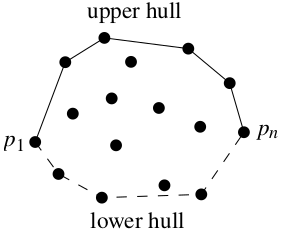
\includegraphics[width=0.5\linewidth]{images/chalgo1.png}
                    \caption{}
                    \label{fig:chalgo1}
                \end{subfigure} &
                \begin{subfigure}{.5\textwidth}
                    \centering
                    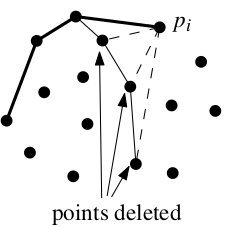
\includegraphics[width=0.5\linewidth]{images/chalgo2.png}
                    \caption{}
                    \label{fig:chalgo2}
                \end{subfigure}
            \end{tabular}
            \caption{Convex Hull Algorithm}
        \end{figure}


        \emph{Input}: A set $P$ of points in a plane.

        \emph{Output}: A list $\mathcal{L}$ cotnaining vertices of $\mathcal{CH}(P)$ in clockwise order. 

        \begin{enumerate}
            \item Sort the points by x-coordinate, resulting in sequence $p_1, ..., p_n$.
            \item Put $p_1$ and $p_2$ in $\mathcal{L}_{up}$, with $p_1$ as the first point. 
            \item \textbf{for} $i \leftarrow 3$ \textbf{to} $n$
            \item \hspace{1cm} \textbf{do} Append $p_i$ to $\mathcal{L}_{up}$
            \item \hspace{2cm} \textbf{while} $| \mathcal{L}_{up} | > 2$ \textbf{and} the last three points in $\mathcal{L}_{up}$ don't make a right turn, 
            \item \hspace{2.5cm} \textbf{do} delete the middle of the last three points in $\mathcal{L}_{up}$
            

            \item Put points $p_{n}$ and $p_{n - 1}$ in $\mathcal{L}_{low}$, with $p_n$ as the first point. 
            \item \textbf{for} $i \leftarrow n - 2$ \textbf{down to} 1
            \item \hspace{1cm} \textbf{do} Append $p_i$ to $\mathcal{L}_{low}$
            \item \hspace{2cm} \textbf{while} $| \mathcal{L}_{low} | > 2$ \textbf{and} the last three points in $\mathcal{L}_{low}$ don't make a right turn, 
            \item \hspace{2.5cm} \textbf{do} delete the middle of the last three points in $\mathcal{L}_{low}$
            
            \item Remove the first and last points from $\mathcal{L}_{low}$ (avoid duplicate points of where upper and lower hull meet).
            \item Append $\mathcal{L}_{low}$ to $\mathcal{L}_{up}$, call the result $\mathcal{L}$
            \item \textbf{return} $\mathcal{L}$
        \end{enumerate}

        \begin{itemize}
            \item We assumed no two points have the same x-coordinate. To consider that, sort same-x-coord points by their y-coord.
            \item We will say for three collinear points (make a straight line), they make a left turn.
            \item Points very close together could create sharp left turns. For these, consider them the same point by rounding.
            \item Algorithm will compute a closed polygonal chain. 
            \item \textbf{Theorem} \emph{The convex hull of a set of n points in the plane can be computed in $O(n \log n)$ time}.
            \item \textbf{Proof}: See \cite{berg08} page 8. 
                \begin{itemize}
                    \item Correctness of computation of upper hull (and lower) is proof by induction. Briefly, the set $\mathcal{L}_{up}$ of $\{p_1, p_2\}$ is trivially the upper hull. $\mathcal{L}_{up}$ containing the chain $\{p_1, ..., p_{i - 1}\}$ is known, by induction to only make right turns, and that all points fall below the chain. When considering point $p_i$, be know that $p_1$ is the smallest point and $p_i$ will be the biggest point thus far. There can be no points above the old chain, because if there were, then it would have to lie between $p_{i-1}$ and $p_i$ in sorted order. 
                    \item Sorting the points can be done in $O(n \log n)$ time. Computing upper hull is done in $O(n)$ time, because the for loop is executed a linear number of times, as any extra executions (from the while loop) is bound by $n$ since extra points can only be deleted onces during the hull construction. Similarly, lower hull construction is $O(n)$ time. Therefore total time for computing convex hull is $O(n \log n)$. 
                \end{itemize}
        \end{itemize}


        \begin{figure}[h]
            \centering
            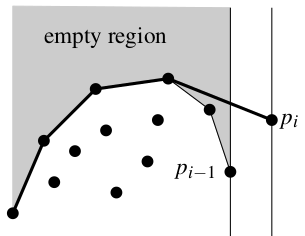
\includegraphics[width=0.3\linewidth]{images/chalgo3.png}
            \caption{Convex Hull Algorithm - Correctness}
            \label{fig:chalgo3}
        \end{figure}
        %%%%%%%%%
        

    %%%
    \subsection{\textbf{Algorithm} Jarvis March (Gift Wrapping) - $O(n^2)$}
    \label{subsec:giftwrapping}
    \url{https://iq.opengenus.org/gift-wrap-jarvis-march-algorithm-convex-hull/}

        \begin{itemize}
            \item Sweepline/Incremental algorithm 
            \item Starting with an extreme point (leftmost/rightmost/etc.), and keep wrapping the points in ccw direction. 
            \item Finding the \emph{next} point involves calculating if the the next candidate makes a ccw orientation with the previous two points. Decide on the directionality, but essentially: 

            \begin{itemize}
                \item Caclulate all the slopes from current point with all the other points. 
                \item Pick the point that gave use the minimum slope. 
                \item The min slope point is now the current point. Repeat this process until we return to the first point. 
                \item \emph{You may need to pick a directionality when you get to the other extreme and start to ``turn around''.}
            \end{itemize}

            \item This algorithm is output sensitive. So runtime is $O(nh)$, and worst is when $h = n$.
        \end{itemize}

    %%%%%%%%%

    %%%
    \subsection{\textbf{Algorithm} Graham Scan - $O(n \log n)$}
    \label{subsec:gscan}
        \url{https://iq.opengenus.org/graham-scan-convex-hull/}

        \begin{itemize}
            \item Uses a stack to remove concavities. Incremental.
            \item Efficient and can run $O(n \log n)$
            \item The runtime rather comes from finding a central position (or even any), calculating all their polar angles (or slopes), and \emph{sorting} them by the angles first. This algorithm comes with a \textbf{Pre-processing} step.
            \item Add the smallest y-coord point to the stack (finding it takes $O(n)$ time), add the next two points in the order to the stack (pre-processing took $O(n\log n)$). Calculate their orientation. The the next point is a candidate; calculate the orientation of the candidate and top two points in the stack. If you get the same orientation, add cancdidate to stack move on to next point; else, pop the stack, and check again. Repeat the popping until you get the orientation desired. Every element is pushed and popped from the stack at most once, and assuming each stack operation takes $O(1)$, so forming the hull is $O(n)$. 
        \end{itemize}
    %%%%%%%%%

    %%%
    \subsection{Bridges}
    \label{subsec:bridge}
        
        \begin{itemize}
            \item A \emph{bridge} is the support line that forms the edge of $\mathcal{CH}$ or one that forms a new $\mathcal{CH}$ edge between two convex polygons when we want to form a new convex hull from their merge. 
            \item Bridge finding is the goal of a divide and conquer method for finding convex hulls.
            \item Bridge finding takes logarithmic time. And there are 8 cases to examine. 
        \end{itemize}

    %%%%%%%%%

    %%%
    \subsection{Divide \& Conquer Convex Hull Methods}
    \label{subsec:dchull}
        
        \begin{itemize}
            \item Typically $T(n) = 2\ T(\frac{n}{2}) + \Theta(n)$. Outline for an unsorted set of points $S$:
                \begin{itemize}
                    \item \emph{assume pre-sort; or sort ($O(n \log n)$)}
                    \item Find $\mathcal{CH}(S, 1, \frac{n}{2})$
                    \item Find $\mathcal{CH}(S, \frac{n}{2} + 1, n)$
                    \item Merge the $\mathcal{CH}$'s
                \end{itemize}
            \item Something like binary search ($O(\log n)$) can be used to find the bridge, for $T(n) = 2\ T(\frac{n}{2}) + \Theta(\log n)$.
            \item Some useful data structures, such as \textbf{concatenable queue}, can make inserting a point, deleting a point, or finding a point, splitting, joining (implant) take time $O(\log n)$.
            \item 
        \end{itemize}

    %%%%%%%%%

    %%%
    \subsection{\textbf{Algorithm} Quick Hull - $O(n^2)$}
    \label{subsec:3dconvexhull}
        \url{https://iq.opengenus.org/quick-hull-convex-hull/}

        \url{https://www.geeksforgeeks.org/quickhull-algorithm-convex-hull/}

        \begin{itemize}
            \item Like quicksort. Divide and Conquer method.
            \item Find the leftmost and rightmost points. 
            \item Find the highest and lowest points relative to the left-right's slope. 
            \item Form a triangle with the left, right, and lowest points. Discard all points inside triangle. 
            \item Repeat this process with one of the left or right, and the extreme point you picked (i.e. one of the edge of the triangle).
            \item Best case is $O(n\log n)$. Worse case is $O(n^2)$.
        \end{itemize}

    
    %%%
    \subsection{\textbf{Algorithm} Ultimate Planar Convex Hull (Marriage Before Conquest ) - $O(n \log h)$}
    \label{subsec:ultimatehull}

    \url{https://iq.opengenus.org/kirkpatrick-seidel-algorithm-convex-hull/}

        \begin{itemize}
            \item Prune \& Search. Output sensitive.
            \item Instead of recurisng on each half after splitting the set like in a D\&C, this computes how the sets should be merged, then recurse on subsets. This finds upper hull, and then when you fid the lower hull, the two sets can be concatenated.
            \item Briefly: \emph{Given a set, find the median vertical. Next goal is to find the bridge that crosses the median vertical. By definition of $\mathcal{CH}$, all points beneath this line is not in the $\mathcal{CH}$, so you discard/prune these points. The remaining points are split into the $L$ and $R$ subsets, and you recurse on them}. 
            \item The Kirkpatrick-Seidel algorithm:
            \begin{enumerate}
                \item \emph{don't sort!}
                % \item Split the points in half, the $L$ set and the $R$ set.
                % \item Find the bridge between $L$ and $R$:
                \item Find the median vertical of the set of points ($T(n) = T(\frac{n}{5}) + T(\frac{2n}{4}) + \Theta(n) = \Theta(n) = \Theta(n)$).
                \item PAIRING: Randomly pair up the points, and calculate the misc. slopes. We have $\frac{n}{2}$ pairs.
                \item Find the median slope ($O(n)$), $m_{\text{median}}$.
                \item Calculate all the y-intercept of all the points if they have slope $m_{\text{median}}$. ``Sweep slope of $m_{\text{median}}$'', and find the most extreme max y-intercept, $b_{\text{max}}$.
                \item BridgeFind: $T_{\text{bridge}}(n) \leq T_{\text{bridge}}(n - \floor*{\frac{n}{4}}) + O(n) = O(n)$
                
                This is when we start removing points that don't meet our criteria:

                \begin{enumerate}
                    \item rotate the line $y_b = m_{\text{median}} x_b + b_{\text{max}}$. Find the bridge with the first point you hit. 
                    \item For the example where $b_{\text{max}}$ is on the right side and has a negative slope for $m_{\text{median}}$, if it his a point that is paired with a point that forms a negative slope, discard the lower point, as you can only ever hit the upper point to be on the hull. Keep all other points. 
                    \item More succinctly, for this pruning step, using the extreme point, $p_{\text{max}}$, you found:
                    \begin{itemize}
                        \item If $p_{\text{max}}$ is on the \emph{right} of line $x_\text{median}$ (where $x_{p_\text{max}} > x_\text{median}$), for every line with a slope less than $m_{\text{median}}$, discard its lower/right point.
                        \item If $p_{\text{max}}$ is on the \emph{left} of line $x_\text{median}$ (where $x_{p_\text{max}} < x_\text{median}$), for every line with a slope greater than $m_{\text{median}}$, discard its upper/left point.
                    \end{itemize}
                    \item This process discards $\frac{1}{4}$ of the points in the set, the pruning. 
                    \item Repeat from the PAIRING step until 2 points are left. These are the points of the Bridge.
                    \begin{equation*}
                        T(n, h) \leq \begin{cases}
                            0 &\text{if } h = 1 \\
                            O(n) &\text{if } h = 2 \\
                            T(\frac{n}{2}, h_l) + T(\frac{n}{2}, h_r) + T_{\text{bridge}}(n) &\text{if } h \geq 3, \\
                            & \text{where } h_l + h_r = h, h_r, h_l \geq 1
                        \end{cases}
                    \end{equation*}

                \end{enumerate}

             

                \item Repeat from step 2 for remainder subsets $L$ and $R$ pm either side of the bridge.
            \end{enumerate}
        \end{itemize}

        \textbf{Proof}

        \emph{Claim:} $T_{\text{bridge}}(n) \leq T_{\text{bridge}}(n - \floor*{\frac{n}{4}}) + O(n)$

        Show by induction on size of $h$ that $T(n, h) \leq c n \log h$. 

        \emph{Basis:} If $h = 2$ (minimum for top hull of the $\mathcal{CH}$), the top edge has at least 2 points. (\emph{$\log 2 = 1$}). $$ T(n, 2) = c_1 n \leq cn \log 2 \hspace{2cm} \text{(pick $c \geq c_1$)}$$

        \emph{Inductive Hypothesis:} $T(n, h) \leq ch \log h$, for $h\leq k$.
        
        \emph{Inductive Step:} 
        \begin{align*}
            T(n, h) &\leq c_1 n + T(\frac{n}{2}, h_l) + T(\frac{n}{2}, h_r) \\
            &\leq c_1 n + \frac{cn}{2} \log h_l + \frac{cn}{2} \log h_r \\
            &\leq c_1 n + \frac{cn}{2} (\log h_l + \log h_r) \\
            &\leq c_1 n + \frac{cn}{2} \log (h_l h_r) \\
            &\leq c_1 n + \frac{cn}{2} \log (h_l (h - h_l)) \\
            &\leq c_1 n + \frac{cn}{2} \log (\frac{h}{2})^2 \\
            &\leq c_1 n + cn \log (\frac{h}{2}) \\
            &\leq c_1 n + cn \log h - cn \log 2\\
            &\leq cn \log h \hspace{2cm} \text{if } c = c_1 \\
        \end{align*}

    %%%%%%%%%

    %%%
    \subsection{\textbf{Algorithm} Dynamic $\mathcal{CH}$ / Order Decomposable Problem - $O(\log^2 n)$}
    \label{subsec:dynamichull}

        \url{https://www.geeksforgeeks.org/dynamic-convex-hull-adding-points-existing-convex-hull/}

        See Dynamic Convex Hull Notes.

        See user guide section on this.

        \begin{itemize}
            \item Order Decomposable Problem, Point Inclusion, Detecting Intersection 
            \item This algorithm addresses when a new point is added to the current set we already computed the convex hull for, or delete a point from the set. This avoids recalculating the entire set for changes regarding single points.
            \item Using a concatenable queue makes bridge finding between two hulls is $O(\log n)$; then we can concatenate the left portion of the left hull with the right portion of the right hull. This relies on sorting the points though, so sorting dominates the runtime at $O(n \log n)$, while the merge gives a recurrance of $T(n) = 2 T(\frac{n}{2}) + O(\log n) = O(n)$.
            \item Best to use a dynamic (augmented) tree as the data structure. The root contains the points of the $\mathcal{CH}$, while the subtrees/node has info about the partial hulls, and can point to another tree. We can retain the info of points that aren's in the $\mathcal{CH}$. The leaves are the actual data/points. 
            \item There are 8 cases to examine to find the bridge between hulls $A$ and $B$. See Class Nodes for Dynamic Convex Hull. But succinctly, when examining if line $\overline{ab}$ could be the bridge, we consider the angles given by $a$ and its neighbors and by $b$ and its neighbors ($\angle a_l\ a\ a_r$ and $\angle b_l\ b\ b_r$), the angles are relative to the line $\overline{ab}$: 
            \begin{enumerate}
                \item $\angle a_l\ a\ a_r$, $\angle b_l\ b\ b_r \leq 180^{\circ}$ (both edges of each angle are above $\overline{ab}$) $\longrightarrow$ $\overline{ab}$ is the bridge.
                \item $\angle b\ a\ a_l \geq 180^{\circ}$ ($\overline{a\ a_l}$ falls ``below'' $\overline{ab}$) $\longrightarrow$ points $a$ and all to the right of $a$ (``above'' $\overline{ab}$) can't be the bridge point, discard. The bridge will be found in $B$ and the left subchain of $A$ from $a$. 
                \item $\angle a\ b\ b_r \geq 180^{\circ}$ ($\overline{b\ b_r}$ falls ``below'' $\overline{ab}$) $\longrightarrow$ points $b$ and all to the left of $b$ (``above'' $\overline{ab}$) can't be the bridge point, discard. The bridge will be found in $A$ and the right subchain of $B$ from $b$. 
                \item Both $\angle a_l\ a\ a_r, \angle a_r\ a\ a_l > 90^{\circ}$ (both $\overline{a\ a_r}$ and $\overline{b\ b_l}$ fall ``below'' $\overline{ab}$, and their vectors extended intersect at point $v = (x, y)$). Let $M_A$ be the max x-coord of $A$, and let $m_B$ be the min x-coord of $B$. There is a region between $M_A$ and $m_B$:
                \begin{enumerate}
                    \item $x < M_A$ and $x < m_B$ ($x$ is to the left of the region), then no points on the left subchain of $A$ including $a$ can be a bridge point. Remove those points.
                    \item $x > m_B$ and $x > M_A$ ($x$ is to the right of the region), then no points on the right subchain of $B$ including $b$ can be a bridge point. Remove those points.
                    \item $M_A < x < m_B$ ($x$ is in the region), then no points on the left subchain of $A$ including $a$ and no points on the right subchain of $B$ including $b$ can be a bridge point. Remove those points.
                \end{enumerate}
                \item Only $\overline{b\ b_l}$ falls below $\overline{ab}$ $\longrightarrow$ discard the right subchain in $A$ and $B$.
                \item Only $\overline{a\ a_r}$ falls below $\overline{ab}$ $\longrightarrow$ discard the left subchain in $A$ and $B$.
            \end{enumerate}
        \end{itemize}

    %%%%%%%%%


    %%%
    \subsection{3D Convex Hull}
    \label{subsec:3dconvexhull}
    Introduced (background) in \cite{berg08} CH. 11
    %%%%%%%%%

    \pagebreak
    % END %%%%%%%%%%%%%%%%%%%%%%%%%%%%%%%%%%%%%%%%%%%%%%%%%%%%%%%%%%%%%%%%%%%%

    % INTERSECTING POINTS %%%%%%%%%%%%%%%%%%%%%%%%%%%%%%%%%%%%%%%%%%%%%%%%%%%%%%%%%%%%%%%%%%%%
    \section{Intersecting Points}
    Covered in \cite{berg08} CH. 2-3, 6

    HW 2

    \subsection{Intro to Intersecting Points}
        \begin{itemize}
            \item Naively find intersecting points of a set $S$ of $n$ line segments is for each segment $s \in S$, find its intersections with all other segments $q \in S$. $O(n^2)$.
            \item We want \emph{output sensitive} or \emph{intersection sensitive} algorithms. 
            \item \textbf{Plane sweep algorithms}: 
                \begin{itemize}
                    \item Uses \emph{status} DS to keep track of lines that currely intersect. It updates when we change the sweep line. The updates happen at \emph{event} or \emph{stopping points}, also kep in a DS. At a stopping point, algorithm updates the status of sweep line, and perform intersection tests. At a point on a line, the start of it when we add it to the status, calculate the intersections of the  line against those lines already in the status DS. Currently, this algorithm is \emph{not} output sensitive.
                    \item Improvements: Only test for intersections on the line with its neighbor lines (at most, test current line against two other lines). This also \emph{orders} the segments in the status DS, so we are delivering the intersection points in order, as well. Stopping point DS now also includes intersection points.  
                \end{itemize}
            \item Special cases to think about later:
                \begin{itemize}
                    \item overlapping lines
                    \item more than two lines intersect at one point 
                    \item line segment has a slope matching the sweeping lstinline
                \end{itemize}    

            \item 
        \end{itemize}

    %%% 
    \subsection{\textbf{Algorithm} Intersections: Plane Sweep}
        \begin{itemize}
            \item Let two lines $\overline{a_0 a_1}$ and $\overline{b_0 b_1}$ intersect at a point $p$. 
            
            \begin{itemize}
                \item Using the sweep line method, there is an event/stopping point \emph{before} $p$ that reveals $\overline{a_0 a_1}$ and $\overline{b_0 b_1}$ are adjacent and therefore get tested for intersection. We are specifically at a point of the sweep line such that i there are no other event points on the sweep line or between the it and the line given by the line's slope and point $p$. When $A$ and $B$ are not yet adjacent, this is when the sweep line is above all the segments, so there is nothing in the status DS. So ther must be an event point $q$ when $A$ and $B$ become adjacent and are tested for intersection.
            \end{itemize}

            \item Stopping points shall include endpoints AND the intersections points calculated along the way that are to the sweeping direction of the sweeping line (no looking backwards at points already detected). 
            \item The status DS shall maintain the ordered sequence of segments that the sweeping line intersects (the stabbing points of sweep line $\ell$).
            \item At a halting point, algorithm must update the status DS and find intersections (if any new). 
            
                \begin{itemize}
                    \item Example (first Endpoint Event): Suppose $s_i$ and $s_k$ are adjacent. The next event is a new line's endpoint of $s_j$. Updating status reveals that $s_j$ is adjacent to $s_i$ and $s_k$. We see that $s_j$ and $s_i$ have an intersecting point, $p$. So we make $p$ a new stopping point. Then move on to next event point. 
                    \item Example (Intersection point event): This is when two lines that intersect cross, so their ordering in the status DS changes. Both shall get at most one new neighbor, for which new intersections must be calculated. Let these be adjacent in order: $s_j\ s_k\ s_l\ s_m$. Let the current event be the intersection of $s_k\ s_l$. $s_k\ s_l$ must switch order, and the new intersections, if any, between new neighbors, $s_j\ s_l$ and $s_k\ s_m$, are calculated and added to the stopping point DS. This can be done if lines were previously found to be adjacent before. 
                    \item Example (second Endpoint Event): Suppose the status order of lines $j\ k\ l$, $k$ is adjacent to its neighbors $j$ and $l$. We reach event of the second endpoint of $k$ (so $k$ shall be leaving status DS). This means $j$ and $l$ will be neighbors and thier intersections gets calculated and put in stopping point DS. 
                \end{itemize}
            
            \item \textbf{Invariant}: All intersection points behind the sweep line have been computed correctly. 
            \item \textbf{Data Structures}:
            
                \begin{itemize}
                    \item \textbf{Stopping Point/Event Point}: Using an event queue or a modified Balanced Binary Search Tree. Ordering will depend on how the $\ell$ sweeps. If $\ell$ is vertical and sweeps along the x-direction, then order by x-coord, and pick the point with the smaller y-coord if two events share the same x. Likewise, if $\ell$ is horizontal and sweeps down the y-direction, then order by y-coord, and pick the point with the smaller x-coord if two points have the same y. Fetching next event and inserting new even is $O(\log m)$ time where $m$ is the number of events. This lets us test whether an event is already in the BBST. During creation (initialization is $O(n\log n)$ for a BBST), we fill the stopping point DS with just endpoints. For each starting endpoint, we store its segment with it. The algorithm runs every time we pop a new event odd and handle it, and runs until the event queue is empty. \emph{See page 26 of \cite{berg08} for full detail on handling all kinds of event points, including degenerates.} 
                    \item \textbf{Status SD}: Using a BBST, which must be dynamic to deal with line segments going in an out as they intersect or stop intersecting $\ell$. The actual ordering will be in the leaves of the BBST. Each update and neighbor operation takes $O(\log n)$
                \end{itemize}
            
            \item Runtime is $O((n + k)\log n)$, where $n$ is the number of segments in the input set, and $k$ is the size of output (we can specify number of intersections, which doesn't double count when more than 2 segments intersects at a common point). 
            \item Status DS is $O(n)$ space. Stopping point DS is $O(n + I)$ space, where $I$ is number of intersections. It may actually be $O(n)$ if we remember to remove intersection points when segments are no longer adjacent, as the intersections will go back in again if they have not been report and their segments become adjacent again later.
        \end{itemize}
        \pagebreak
    %%%%%%%%%%%%%%%%%%%%%%%

    %%%%%%%%%%%%%%%%%%%%%%%
    \subsection{Doubly Connected Edge List}
        \begin{itemize}
            \item DCEL contains a record for each face, edge, and vertex of a planar subdivision. (In application, it is useful for these records to also contain attribute information, such as what is in a given face.)
        \end{itemize}
    \pagebreak
    %%%%%%%%%%%%%%%%%%%%%%%

    %%%%%%%%%%%%%%%%%%%%%%%
    \section{Polygon Triangulation}
    See CH. 3 of \cite{berg08}

    HW 2

    \subsection{Art Gallery Problem with 3-coloring Approach - $O(n\log n)$}
        \begin{itemize}
            \item For triangulation of the polygon, it should deliver a DCEL, which allows for constant time stepping into another triangle/face of the triangulated polygon. This should be $O(n\log n)$ time.
            \item Depth-first search can be used to compute the 3-coloring of the vertices of all the triangles, which should take $O(n)$ time.
            \item There are at most $\floor*{n / 3}$ camera placements to find in a polygon of $n$ vertices. The worst case being the comb-shaped polygon.
        \end{itemize}
    \pagebreak
    %%%%%%%%%%%%%%%%%%%%%%%

    %%%%%%%%%%%%%%%%%%%%%%%
    \subsection{Triangulation: Partitioning a Polygon into Monotone Pieces}

        \begin{itemize}
            \item $O(n^2)$ if we take $O(n)$ for each vertex to find a proper diagonal to make a triangle. 
            \item $O(n)$ is we know polygon is convex, so we simply take the segments from one vertex to all other vertices, and we have our triangulation.
            \item Potential but hard strategy is to decompose the polygon into convex polygons and triangluate the sub-convex-polygons. However, we instead take an easier strategy: Decompose the polygon into monotone pieces, and triangulate those. 
            
                \begin{itemize}
                    \item Partition into (y-)Montone pieces with diagonals: When walking from the topmost to bottomost vertices, we detect the direction we are going, namely dowards. A turn vertex is when the direction changes. So at that vertex, if the two incident edges of the turn vertex lie below it and the interior of the polygon above it, then the diagnonal for $v$ must be above $v$. Likewise, if the two incident edges of $v$ lie above $v$, then the diagonal should be below $v$. See page 50 in \cite{berg08}
                \end{itemize}

        \end{itemize}
    \pagebreak
    %%%%%%%%%%%%%%%%%%%%%%%
    
    % END %%%%%%%%%%%%%%%%%%%%%%%%%%%%%%%%%%%%%%%%%%%%%%%%%%%%%%%%%%%%%%%%%%%%
   

    \pagebreak
    %%%%%%%%%%%%%%%%%%%%%%%%%%%%%%%%%%%%%%%%%%%%%%%%%%%%%%%%%%%%%%%%%%%%%
    \begin{thebibliography}{1}
        \bibitem[1]{berg08}Mark de Berg, Otfried Cheong, Marc van Kreveld, and Mark Overmars. 2008. Computational Geometry: Algorithms and Applications (3rd ed. ed.). Springer-Verlag TELOS, Santa Clara, CA, USA.
        \bibitem[2]{key2}Hi
    \end{thebibliography}
    % END %%%%%%%%%%%%%%%%%%%%%%%%%%%%%%%%%%%%%%%%%%%%%%%%%%%%%%%%%%%%%%%%%%%%

\end{document}